\RequirePackage{atbegshi}
\documentclass{beamer}

\usepackage{graphicx,epstopdf,subfigure,booktabs,natbib}
\usepackage{tikz}
\usetikzlibrary{arrows,shapes,positioning,trees,mindmap,backgrounds}

%\usetheme[compress,subsection=F]{Singapore}
%\useoutertheme[subsection=false]{miniframes}
\usetheme[hideallsubsections]{Hannover}
%\usecolortheme{dove}
\usecolortheme{seagull}
\useinnertheme{default}

\bibliographystyle{plainnat}
\bibpunct{[}{]}{;}{a}{}{,}
\usefonttheme{serif}
\usepackage{mathpazo}

\definecolor[named]{Yellow}{cmyk}{.01,.11,.74,0}
\definecolor[named]{Red}{cmyk}{0,.48,.62,0}
\definecolor[named]{Green}{cmyk}{.31,0,.69,0}
\definecolor[named]{Teal}{cmyk}{.39,.05,.18,0}
\definecolor[named]{Purple}{cmyk}{.16,.31,0,0}
\definecolor[named]{Gray}{cmyk}{0,0,0,.29}

\tikzset{em/.style ={
        fill=Yellow,
        draw=black,
		thick, 
    },
    brackish/.style={
        fill=Red, 
        draw=black,
		thick,
    },
    ox/.style={
        fill=Green,
        draw=black,
		thick, 
    },
    contact/.style={
        fill=Purple,
        draw=black,
		thick, 
    },
    tm/.style={
        fill=Teal, 
        draw=black,
		thick,
    },    
    txt/.style ={
		text width=5em,
		text centered
    },
    pump/.style ={
        draw,
        thick,
        double distance=1pt,
        -latex'
    },
    gravity/.style ={
        draw,
        thick,
        -stealth,
    },
    double/.style ={
        draw,
        thick,
        stealth-stealth,
    },
    phantom/.style = {
    		none,
    	    inner sep=-10,
		outer sep=1pt,
		node distance=1mm
	}}

\title[\scshape Probabalistic Midterm Model]{Experiences with Policy Development and Forecasting for the Midterm Probabilistic Model}
%\subtitle{Past, Present and Future Work}
\author[\it Cameron Bracken]{Cameron Bracken\\M.S. Student\\CADSWES, CU Boulder}
\date{Febrary 11th, 2010}

\begin{document}

%%%%%%%%%%%%%%%%%%%%%%%%%%%%%%%%%%%%%%%%%%%%%%%%%%%%%%
%%%%%%%%%%%%%%%%%%%%%%%%%%%%%%%%%%%%%%%%%%%%%%%%%%%%%%
\begin{frame}
\titlepage
\end{frame}

%%%%%%%%%%%%%%%%%%%%%%%%%%%%%%%%%%%%%%%%%%%%%%%%%%%%%%
%%%%%%%%%%%%%%%%%%%%%%%%%%%%%%%%%%%%%%%%%%%%%%%%%%%%%%
\section{24 Month Study}
\begin{frame}{24 Month Study}
\begin{itemize}
	\item BOR's Monthly midterm operational forecast model for the CRB
	\item Inputs: 
		\begin{itemize}
			\item Unregulated inflows (RFC $\sim$1 year, climatology after)
			\item Releases manually input by individual dam operators
		\end{itemize}
	\item Outputs: 
	\begin{itemize}
		\item Power, Evap, Elevation, Storage, etc. 
	\end{itemize}
\end{itemize}
\end{frame}

%%%%%%%%%%%%%%%%%%%%%%%%%%%%%%%%%%%%%%%%%%%%%%%%%%%%%%
%%%%%%%%%%%%%%%%%%%%%%%%%%%%%%%%%%%%%%%%%%%%%%%%%%%%%%
\section{Probabilistic Midterm Model}
\begin{frame}{Probabilistic Midterm Model}
\begin{itemize}
\item Midterm operational forecast model for the CRB
\item Probablistic version 24 month study
\item New features
\end{itemize}
\pause

\begin{center}
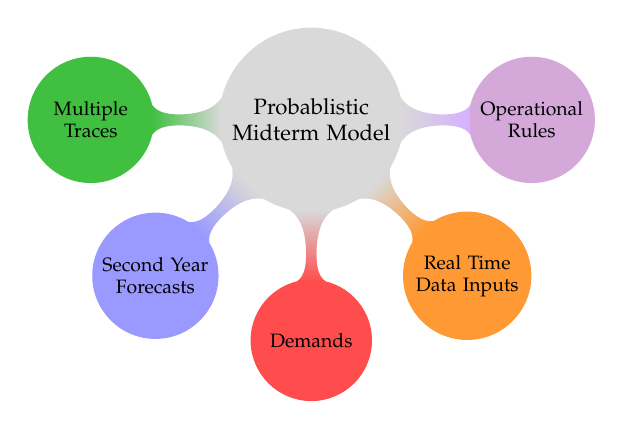
\begin{tikzpicture} [small mindmap,level 1 concept/.append style={sibling angle=45}]
	\path[mindmap,concept color=gray!30] 
		node[concept] {Probablistic Midterm Model} [counterclockwise from=180] 
			child[concept color=green!50!gray] { node[concept] {Multiple Traces} }
			child[concept color=blue!40] { node[concept] {Second Year Forecasts} 
				% [clockwise from=-30] 
				%	child[concept color=purple!40] { node[concept] {Operational Mode} } 
				%	child[concept color=purple!40] { node[concept] {Analysis Mode} }
			} 
			child[concept color=red!70] { node[concept] {Demands} }
			child[concept color=orange!80] { node[concept] {Real Time Data Inputs} }
			child[concept color=Purple] { node[concept] {Operational Rules} 
		}; 
\end{tikzpicture} 
\end{center}

\end{frame}

%%%%%%%%%%%%%%%%%%%%%%%%%%%%%%%%%%%%%%%%%%%%%%%%%%%%%%
%%%%%%%%%%%%%%%%%%%%%%%%%%%%%%%%%%%%%%%%%%%%%%%%%%%%%%
\section{Modeling Operations}
\begin{frame}{Modeling Operations}

\begin{itemize}
	\item Actual operations are a combination of many factors:
	
	\begin{itemize}
		\item Law (EIS's)
		\item Guidelines (Power Generation)
		\item Daily Targets
		\item Monthly or Seasonal Targets
		\item Peak Flows
		\item Base Flow
		\item Extreme Events (Dam Safety Operations)
		\item MANY More...
	\end{itemize}
\end{itemize}
\end{frame}



%%%%%%%%%%%%%%%%%%%%%%%%%%%%%%%%%%%%%%%%%%%%%%%%%%%%%%
%%%%%%%%%%%%%%%%%%%%%%%%%%%%%%%%%%%%%%%%%%%%%%%%%%%%%%
\section{Rules Development}
\begin{frame}{Rules Development: From Management to Model}
For Each Reservoir:

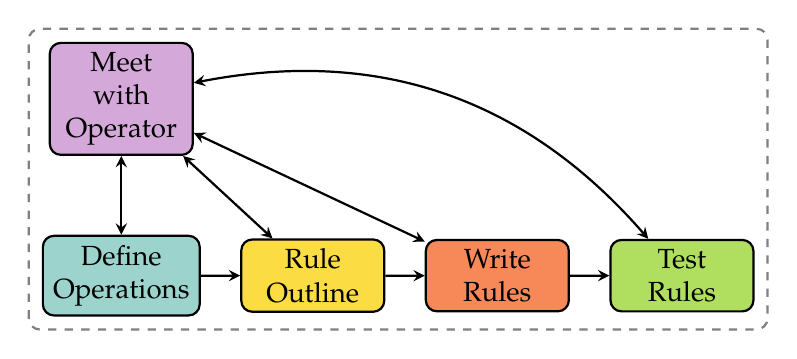
\begin{tikzpicture}
    [
    node distance=10mm and 5mm,
    scale=.6,
    text width=4.5em,
    text centered,
    rectangle,
    rounded corners,
    show background rectangle,
    background rectangle/.style={
		draw=gray,
		thick,
		dashed,
		rounded corners
	}
    ]

    \node(meet) [contact] {Meet with Operator};
    \pause
    
    \node(define) [tm,below=of meet,text width=5em] {Define Operations};
    \path[double] (meet) -- (define);
    \pause 
    
    \node(outline) [em,right=of define] {Rule Outline};
    \path[gravity] (define) -- (outline);
    \pause
    
    \path[double] (meet) -- (outline);
    \pause
    
    \node(rules) [brackish,right=of outline] {Write Rules};
    \path[gravity] (outline) -- (rules);
    \pause
    
    \path[double] (meet) -- (rules);
    \pause
    
    \node(test) [ox,right=of rules] {Test Rules};
    \path[gravity] (rules) -- (test);
	\pause
	
	\path[double] (meet) edge[bend left] (test);
    \pause
	
\end{tikzpicture}
\end{frame}

%%%%%%%%%%%%%%%%%%%%%%%%%%%%%%%%%%%%%%%%%%%%%%%%%%%%%%
%%%%%%%%%%%%%%%%%%%%%%%%%%%%%%%%%%%%%%%%%%%%%%%%%%%%%%
\section{Implications}
\begin{frame}{Implications}
\begin{itemize}
\item Self-documenting process
\item Testing gets harder as more reservoirs are added
\item Many operations don't translate perfectly to a monthly model

\item Rules must be very robust for different model start dates and hydrologic conditions
\begin{itemize}
\item Lots of checking which month it is!
\end{itemize}
\item ...3,2,1 rule ordering is crucial
\end{itemize}
\end{frame}

%%%%%%%%%%%%%%%%%%%%%%%%%%%%%%%%%%%%%%%%%%%%%%%%%%%%%%
%%%%%%%%%%%%%%%%%%%%%%%%%%%%%%%%%%%%%%%%%%%%%%%%%%%%%%
\section{Conclusions}
\begin{frame}{Conclusions}
\begin{itemize}
\item Fontenelle Rules written 
\item Flaming Gorge Rules in progress
\item Aspinall and Navajo are on the horizon
\end{itemize}
\end{frame}

\section{~}

\end{document}  